\documentclass[11pt,a4paper]{report}
\usepackage[textwidth=37em,vmargin=30mm]{geometry}
\usepackage{calc,xunicode,amsmath,amssymb,paralist,enumitem,tabu,booktabs,datetime2,xeCJK,xeCJKfntef,listings}
\usepackage{tocloft,fancyhdr,tcolorbox,xcolor,graphicx,eso-pic,xltxtra,xelatexemoji}

\newcommand{\envyear}[0]{2025}
\newcommand{\envdatestr}[0]{2025-04-21}
\newcommand{\envfinaldir}[0]{webdb/2025/20250421/final}

\usepackage[hidelinks]{hyperref}
\hypersetup{
    colorlinks=false,
    pdfpagemode=FullScreen,
    pdftitle={Web Digest - \envdatestr}
}

\setlength{\cftbeforechapskip}{10pt}
\renewcommand{\cftchapfont}{\rmfamily\bfseries\large\raggedright}
\setlength{\cftbeforesecskip}{2pt}
\renewcommand{\cftsecfont}{\sffamily\small\raggedright}

\setdefaultleftmargin{2em}{2em}{1em}{1em}{1em}{1em}

\usepackage{xeCJK,xeCJKfntef}
\xeCJKsetup{PunctStyle=plain,RubberPunctSkip=false,CJKglue=\strut\hskip 0pt plus 0.1em minus 0.05em,CJKecglue=\strut\hskip 0.22em plus 0.2em}
\XeTeXlinebreaklocale "zh"
\XeTeXlinebreakskip = 0pt


\setmainfont{Brygada 1918}
\setromanfont{Brygada 1918}
\setsansfont{IBM Plex Sans}
\setmonofont{JetBrains Mono NL}
\setCJKmainfont{Noto Serif CJK SC}
\setCJKromanfont{Noto Serif CJK SC}
\setCJKsansfont{Noto Sans CJK SC}
\setCJKmonofont{Noto Sans CJK SC}

\setlength{\parindent}{0pt}
\setlength{\parskip}{8pt}
\linespread{1.15}

\lstset{
	basicstyle=\ttfamily\footnotesize,
	numbersep=5pt,
	backgroundcolor=\color{black!5},
	showspaces=false,
	showstringspaces=false,
	showtabs=false,
	tabsize=2,
	captionpos=b,
	breaklines=true,
	breakatwhitespace=true,
	breakautoindent=true,
	linewidth=\textwidth
}






\newcommand{\coverpic}[2]{
    % argv: itemurl, authorname
    Cover photo by #2~~(\href{#1}{#1})
}
\newcommand{\makeheader}[0]{
    \begin{titlepage}
        % \newgeometry{hmargin=15mm,tmargin=21mm,bmargin=12mm}
        \begin{center}
            
            \rmfamily\scshape
            \fontspec{BaskervilleF}
            \fontspec{Old Standard}
            \fontsize{59pt}{70pt}\selectfont
            WEB\hfill DIGEST
            
            \vfill
            % \vskip 30pt
            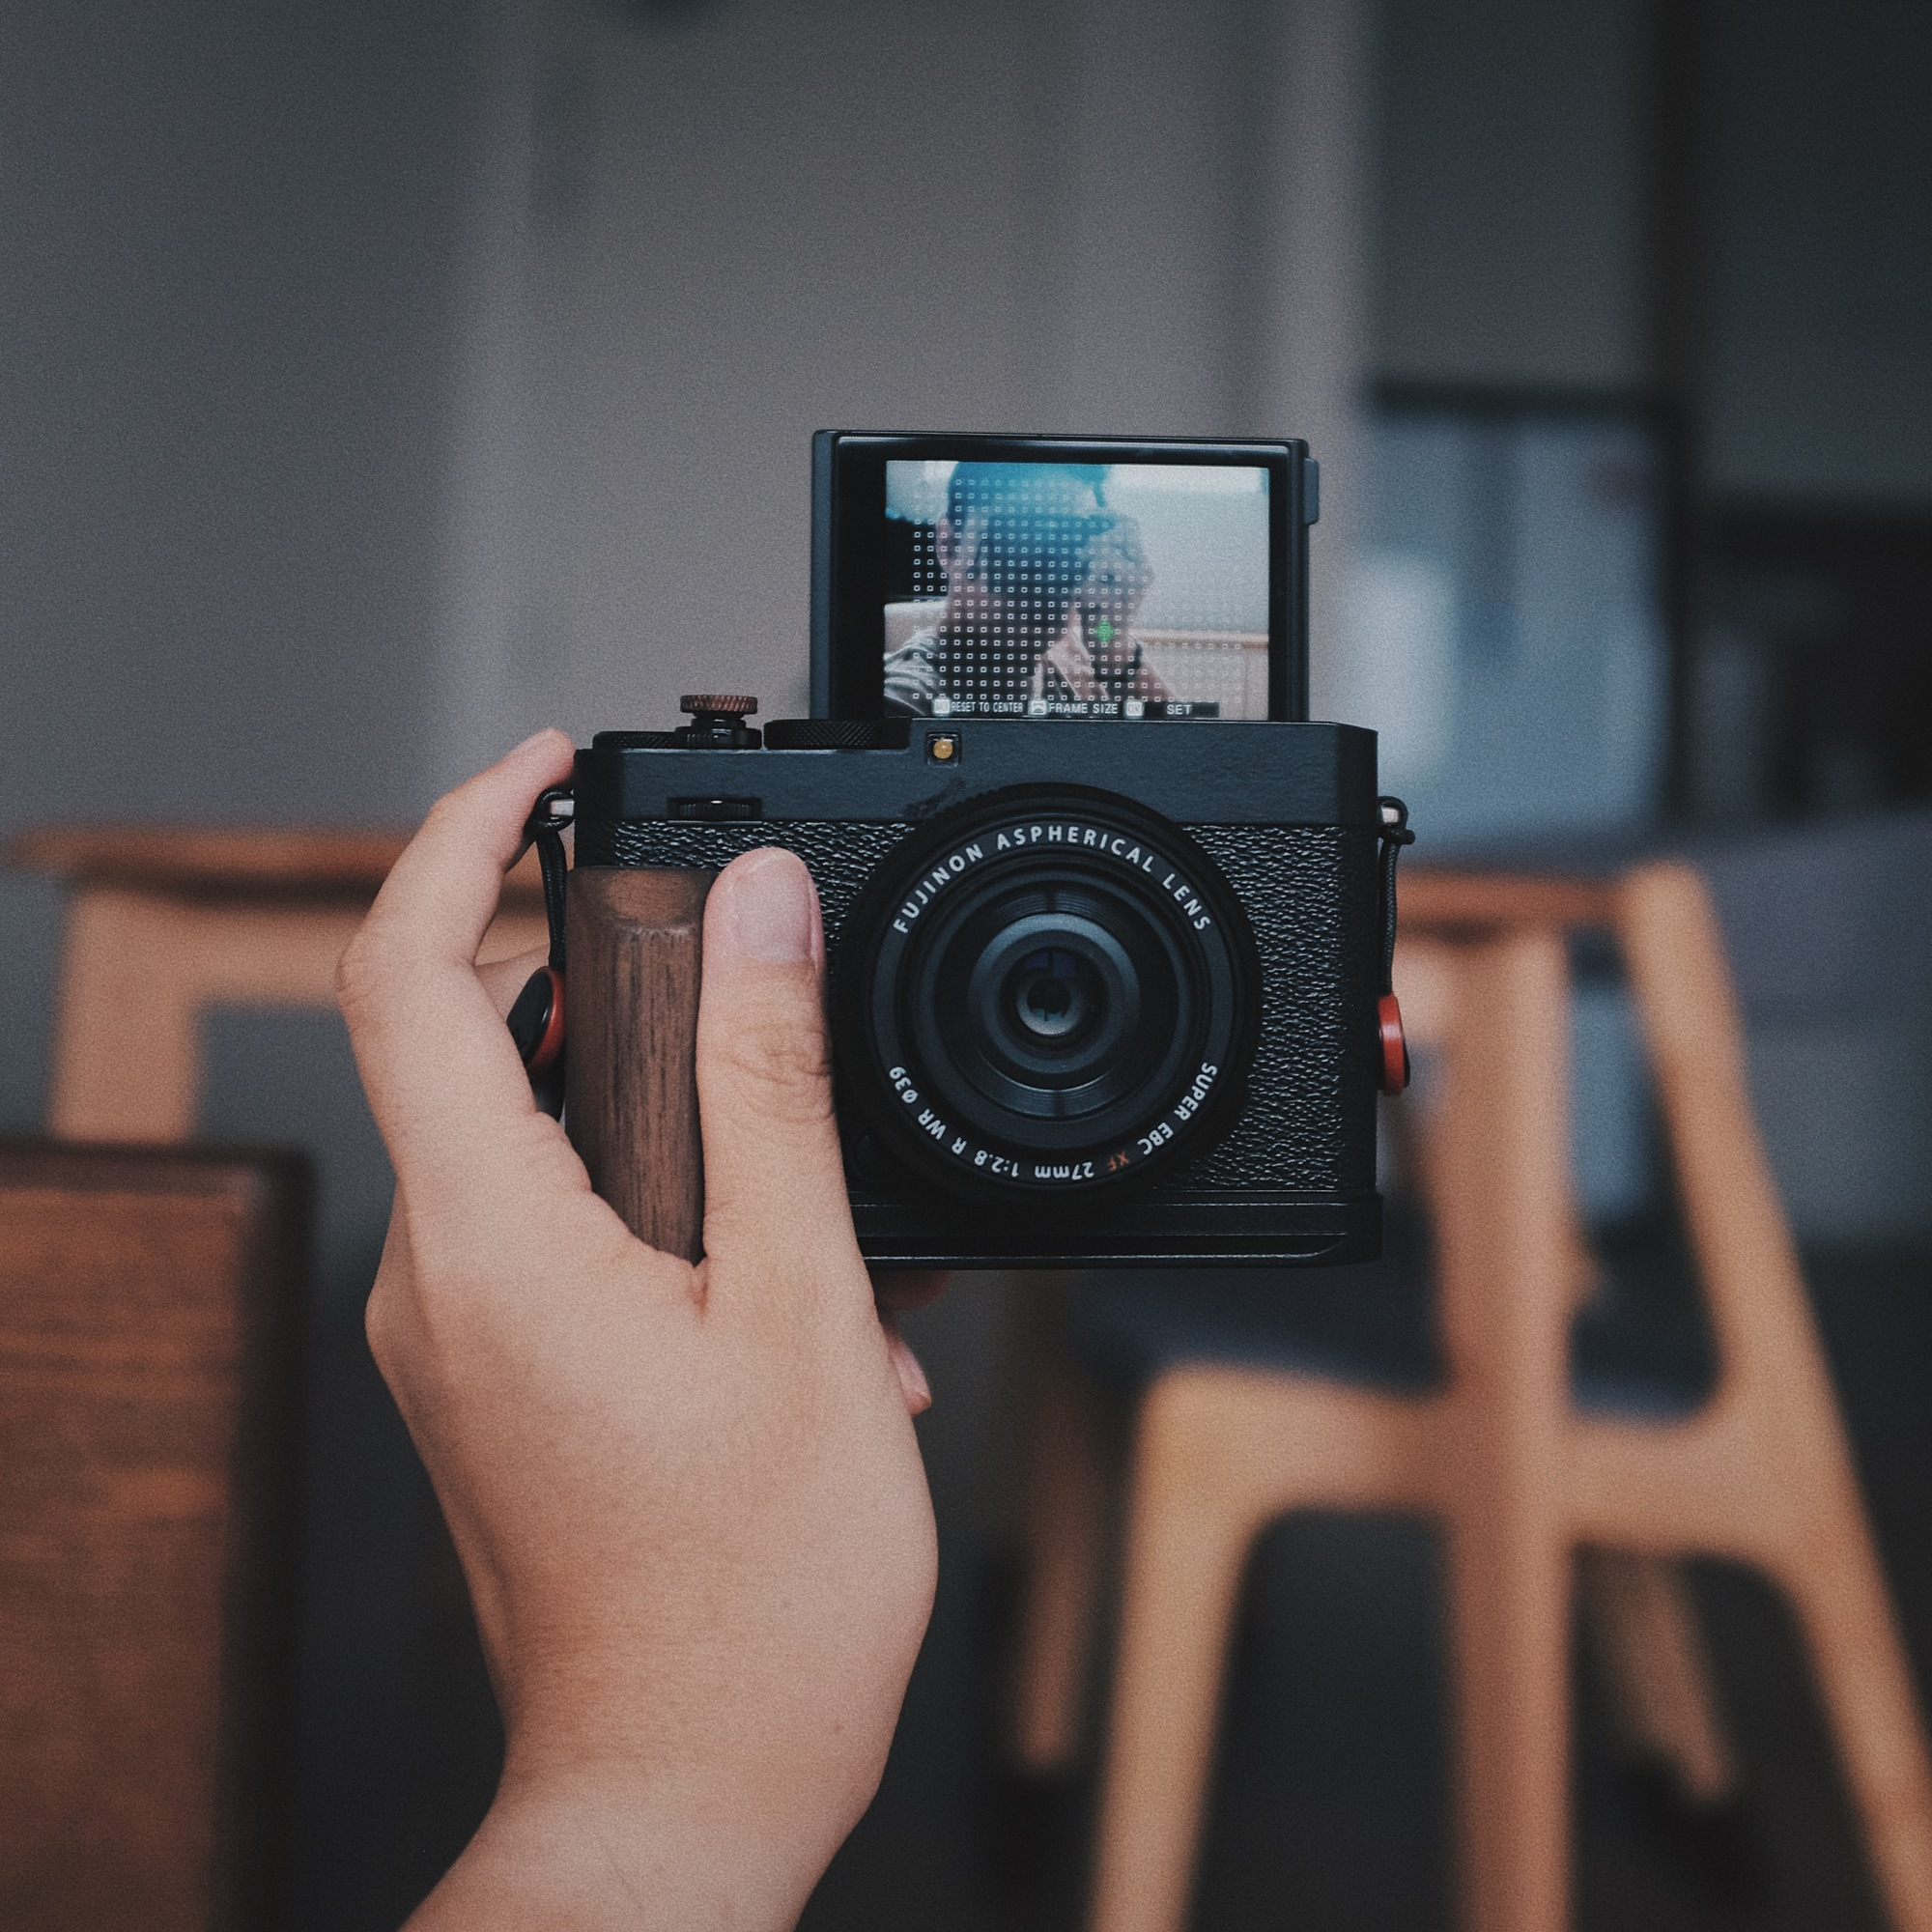
\includegraphics[width=\linewidth]{\envfinaldir/coverpic-prod.jpg}\par
            % \vskip 30pt
            \vfill

            \normalsize\rmfamily\scshape
            \copyright{} The Web Digest Project \hfill\large \envdatestr
        \end{center}
    \end{titlepage}
    % \restoregeometry
}
\newcommand{\simplehref}[1]{%
    \textcolor{blue!80!green}{\href{#1}{#1}}%
}
\renewcommand{\contentsname}{\center\Huge\sffamily\bfseries Contents\par\vskip 20pt}
\newcounter{ipartcounter}
\setcounter{ipartcounter}{0}
\newcommand{\ipart}[1]{
    % \vskip 20pt
    \clearpage
    \stepcounter{ipartcounter}
    \phantomsection
    \addcontentsline{toc}{chapter}{#1}
    % \begin{center}
    %     \Huge
    %     \sffamily\bfseries
    %     #1
    % \end{center}
    % \vskip 20pt plus 7pt
}
\newcounter{ichaptercounter}
\setcounter{ichaptercounter}{0}
\newcommand{\ichapter}[1]{
    % \vskip 20pt
    \clearpage
    \stepcounter{ichaptercounter}
    \phantomsection
    \addcontentsline{toc}{section}{\numberline{\arabic{ichaptercounter}}#1}
    \begin{center}
        \Huge
        \sffamily\bfseries
        #1
    \end{center}
    \vskip 20pt plus 7pt
}
\newcommand{\entrytitlefont}[1]{\subsection*{\raggedright\Large\sffamily\bfseries#1}}
\newcommand{\entryitemGeneric}[2]{
    % argv: title, url
    \parbox{\linewidth}{
        \entrytitlefont{#1}\par\vskip 5pt
        \footnotesize\ttfamily\mdseries
        \simplehref{#2}
    }\vskip 11pt plus 11pt minus 1pt
}
\newcommand{\entryitemGithub}[3]{
    % argv: title, url, desc
    \parbox{\linewidth}{
        \entrytitlefont{#1}\par\vskip 5pt
        \footnotesize\ttfamily\mdseries
        \simplehref{#2}\par\vskip 5pt
        \small\rmfamily\mdseries#3
    }\vskip 11pt plus 11pt minus 1pt
}
\newcommand{\entryitemAp}[3]{
    % argv: title, url, desc
    \parbox{\linewidth}{
        \entrytitlefont{#1}\par\vskip 5pt
        \footnotesize\ttfamily\mdseries
        \simplehref{#2}\par\vskip 5pt
        \small\rmfamily\mdseries#3
    }\vskip 11pt plus 11pt minus 1pt
}
\newcommand{\entryitemHackernews}[3]{
    % argv: title, hnurl, rawurl
    % \parbox{\linewidth}{
    %     \entrytitlefont{#1}\par\vskip 5pt
    %     \footnotesize\ttfamily\mdseries
    %     \simplehref{#3}\par
    %     \textcolor{black!50}{\href{#2}{#2}}
    % }\vskip 11pt plus 11pt minus 1pt
    \begin{minipage}{\linewidth}
            \entrytitlefont{#1}\par\vskip 5pt
            \footnotesize\ttfamily\mdseries
            \simplehref{#3}\par
            \textcolor{black!50}{\href{#2}{#2}}
    \end{minipage}\par\vskip 11pt plus 11pt minus 1pt
}







\begin{document}

\makeheader

\tableofcontents\clearpage




\ipart{Developers}
\ichapter{Hacker News}
\entryitemTwoLinks{Show HN: JuryNow – Get an anonymous instant verdict from 12 real people}{https://news.ycombinator.com/item?id=43745554}{https://jurynow.app/}

\entryitemTwoLinks{U.S. citizen in Arizona detained by immigration officials for 10 days}{https://news.ycombinator.com/item?id=43745469}{https://news.azpm.org/p/news-articles/2025/4/18/224512-us-citizen-in-arizona-detained-by-immigration-officials-for-10-days/}

\entryitemTwoLinks{First hormone-free male birth control pill enters human trials}{https://news.ycombinator.com/item?id=43745296}{https://scitechdaily.com/99-effective-first-hormone-free-male-birth-control-pill-enters-human-trials/}

\entryitemTwoLinks{The movie mistake mystery from "Revenge of the Sith"}{https://news.ycombinator.com/item?id=43745141}{https://fxrant.blogspot.com/2025/04/the-movie-mistake-mystery-from-revenge.html}

\entryitemTwoLinks{Things Zig comptime won't do}{https://news.ycombinator.com/item?id=43744591}{https://matklad.github.io/2025/04/19/things-zig-comptime-wont-do.html}

\entryitemTwoLinks{The skill of the future is not 'AI', but 'Focus'}{https://news.ycombinator.com/item?id=43744394}{https://www.carette.xyz/posts/focus\_will\_be\_the\_skill\_of\_the\_future/}

\entryitemTwoLinks{Jagged AGI: o3, Gemini 2.5, and everything after}{https://news.ycombinator.com/item?id=43744173}{https://www.oneusefulthing.org/p/on-jagged-agi-o3-gemini-25-and-everything}

\entryitemTwoLinks{Why is OpenAI buying Windsurf?}{https://news.ycombinator.com/item?id=43743993}{https://theahura.substack.com/p/tech-things-openai-buys-windsurf}

\entryitemTwoLinks{The Joy of Linux Theming in the Age of Bootable Containers}{https://news.ycombinator.com/item?id=43743784}{https://blues.win/posts/joy-of-linux-theming/}

\entryitemTwoLinks{Gemma 3 QAT Models: Bringing AI to Consumer GPUs}{https://news.ycombinator.com/item?id=43743337}{https://developers.googleblog.com/en/gemma-3-quantized-aware-trained-state-of-the-art-ai-to-consumer-gpus/}

\entryitemTwoLinks{100 Years to Solve an Integral (2020)}{https://news.ycombinator.com/item?id=43741273}{https://liorsinai.github.io/mathematics/2020/08/27/secant-mercator.html}

\entryitemTwoLinks{Pretty State Machine Patterns in Rust (2016)}{https://news.ycombinator.com/item?id=43741051}{https://hoverbear.org/blog/rust-state-machine-pattern/}

\entryitemTwoLinks{Novel color via stimulation of individual photoreceptors at population scale}{https://news.ycombinator.com/item?id=43741013}{https://www.science.org/doi/10.1126/sciadv.adu1052}

\entryitemTwoLinks{Layered Design in Go}{https://news.ycombinator.com/item?id=43740992}{https://jerf.org/iri/post/2025/go\_layered\_design/}

\entryitemTwoLinks{A unique sound alleviates motion sickness}{https://news.ycombinator.com/item?id=43740021}{https://www.nagoya-u.ac.jp/researchinfo/result-en/2025/04/20250408-01.html}

\entryitemTwoLinks{Ultrathink is a Claude Code a magic word}{https://news.ycombinator.com/item?id=43739997}{https://simonwillison.net/2025/Apr/19/claude-code-best-practices/}

\entryitemTwoLinks{Electromagnetism as a Purely Geometric Theory}{https://news.ycombinator.com/item?id=43739529}{https://iopscience.iop.org/article/10.1088/1742-6596/2987/1/012001}

\entryitemTwoLinks{Show HN: I built an AI that turns GitHub codebases into easy tutorials}{https://news.ycombinator.com/item?id=43739456}{https://github.com/The-Pocket/Tutorial-Codebase-Knowledge}

\entryitemTwoLinks{The Art of Assembly Language (2010)}{https://news.ycombinator.com/item?id=43739285}{https://www.plantation-productions.com/Webster/www.artofasm.com/Linux/HTML/AoATOC.html}

\entryitemTwoLinks{Vibe Coding is not an excuse for low-quality work}{https://news.ycombinator.com/item?id=43739037}{https://addyo.substack.com/p/vibe-coding-is-not-an-excuse-for}\ichapter{Phoronix}
\entryitemGeneric{\hskip 0pt{}Linux 6.15-rc3 Released With GCC 15 Build Fixes, Intel Bartlett Lake \& Zen 5 Check}{https://www.phoronix.com/news/Linux-6.15-rc3-Released}

\entryitemGeneric{\hskip 0pt{}NVIDIA Engineer Posts New NOVA Driver Patches - Still Far From Doing Anything Useful}{https://www.phoronix.com/news/NOVA-16-Patches-Still-Early}

\entryitemGeneric{\hskip 0pt{}Sway 1.11-rc1 Released With Many New Features \& New Wayland Protocols}{https://www.phoronix.com/news/Sway-1.11-rc1-Released}

\entryitemGeneric{\hskip 0pt{}FreeType Fixes Inefficient Code Causing 10x Startup Time Hit When Loading Arial TTF Font}{https://www.phoronix.com/news/FreeType-Slow-Loading-Arial-TTF}

\entryitemGeneric{\hskip 0pt{}Linux 6.13 Series Ends With The Linux 6.13.12 Release}{https://www.phoronix.com/news/Linux-6.13-Ends}

\entryitemGeneric{\hskip 0pt{}OpenVPN DCO Driver Queued In Net-Next Ahead Of Linux 6.16}{https://www.phoronix.com/news/OpenVPN-DCO-In-Net-Next-6.16}

\entryitemGeneric{\hskip 0pt{}HFS/HFS+ File-System Driver Support For Linux May End Up Being Maintained}{https://www.phoronix.com/news/Apple-HFS-2025-Linux-Maintain}

\entryitemGeneric{\hskip 0pt{}Intel Simplifies Its Firmware License For The Integrated Sensor Hub "ISH"}{https://www.phoronix.com/news/Intel-ISH-Simplified-Firmware}

\entryitemGeneric{\hskip 0pt{}FFmpeg AV1 Vulkan Encoder Patch Posted}{https://www.phoronix.com/news/FFmpeg-AV1-Vulkan-Encoder}\ichapter{Dribbble}
\entryitemGeneric{\hskip 0pt{}Tanuki - Raccoon, Animal Logo Design}{https://dribbble.com/shots/25917338-Tanuki-Raccoon-Animal-Logo-Design}

\entryitemGeneric{\hskip 0pt{}Cruising for the coast}{https://dribbble.com/shots/25914452-Cruising-for-the-coast}

\entryitemGeneric{\hskip 0pt{}Case study: Educational Website on Space Pollution}{https://dribbble.com/shots/25914349-Case-study-Educational-Website-on-Space-Pollution}

\entryitemGeneric{\hskip 0pt{}Columbus Rapids®}{https://dribbble.com/shots/25915181-Columbus-Rapids}

\entryitemGeneric{\hskip 0pt{}UNIC // Mobile App}{https://dribbble.com/shots/25913185-UNIC-Mobile-App}

\entryitemGeneric{\hskip 0pt{}Phantom concept with Widget}{https://dribbble.com/shots/25911511-Phantom-concept-with-Widget}

\entryitemGeneric{\hskip 0pt{}Cute Easter Bunny Mascot}{https://dribbble.com/shots/25914543-Cute-Easter-Bunny-Mascot}

\entryitemGeneric{\hskip 0pt{}Startup Branding for Holidu: visual identity, brand design}{https://dribbble.com/shots/25903662-Startup-Branding-for-Holidu-visual-identity-brand-design}

\entryitemGeneric{\hskip 0pt{}Mountains to Sea}{https://dribbble.com/shots/25910072-Mountains-to-Sea}

\entryitemGeneric{\hskip 0pt{}Forg Logo}{https://dribbble.com/shots/25910287-Forg-Logo}

\entryitemGeneric{\hskip 0pt{}Cute Unicorn Mascot}{https://dribbble.com/shots/25909768-Cute-Unicorn-Mascot}

\entryitemGeneric{\hskip 0pt{}Logolounge Book 15 Entry - Client Work}{https://dribbble.com/shots/25909344-Logolounge-Book-15-Entry-Client-Work}

\entryitemGeneric{\hskip 0pt{}Reindeer in Golden Light 🦌}{https://dribbble.com/shots/25905633-Reindeer-in-Golden-Light}

\entryitemGeneric{\hskip 0pt{}Altitude}{https://dribbble.com/shots/25902364-Altitude}

\entryitemGeneric{\hskip 0pt{}Automation builder - Wireframes}{https://dribbble.com/shots/25904187-Automation-builder-Wireframes}

\entryitemGeneric{\hskip 0pt{}Logo Collection > Birds Volume 03}{https://dribbble.com/shots/25905911-Logo-Collection-Birds-Volume-03}

\entryitemGeneric{\hskip 0pt{}Details - Amplemarket Logo \& Visual Identity}{https://dribbble.com/shots/25904732-Details-Amplemarket-Logo-Visual-Identity}

\entryitemGeneric{\hskip 0pt{}LogoLounge Book 15 Entry}{https://dribbble.com/shots/25904019-LogoLounge-Book-15-Entry}

\entryitemGeneric{\hskip 0pt{}FarmGirl Fresh®}{https://dribbble.com/shots/25905838-FarmGirl-Fresh}

\entryitemGeneric{\hskip 0pt{}Road Tripping}{https://dribbble.com/shots/25900418-Road-Tripping}

\entryitemGeneric{\hskip 0pt{}Lion sketches}{https://dribbble.com/shots/25898381-Lion-sketches}

\entryitemGeneric{\hskip 0pt{}Bloksy Logo Design - City, Colorful, Building, Construction}{https://dribbble.com/shots/25898764-Bloksy-Logo-Design-City-Colorful-Building-Construction}

\entryitemGeneric{\hskip 0pt{}Cute Shiba Catching a Ball}{https://dribbble.com/shots/25900210-Cute-Shiba-Catching-a-Ball}

\entryitemGeneric{\hskip 0pt{}Corti: Visual identity exploration}{https://dribbble.com/shots/25899331-Corti-Visual-identity-exploration}


\ipart{Developers~~~~(zh-Hans)}
\ichapter{Solidot}
\entryitemGeneric{\hskip 0pt{}Arch Linux 成为最新一个用 Valkey 取代 Redis 的发行版}{https://www.solidot.org/story?sid=81095}

\entryitemGeneric{\hskip 0pt{}CA/Browser Forum 投票到 2029 年将证书有效期缩短至 47 天}{https://www.solidot.org/story?sid=81094}

\entryitemGeneric{\hskip 0pt{}研究发现五成员工使用未批准的 AI 工具}{https://www.solidot.org/story?sid=81093}

\entryitemGeneric{\hskip 0pt{}OpenAI 新推理模型有更高的幻觉比例}{https://www.solidot.org/story?sid=81092}

\entryitemGeneric{\hskip 0pt{}机器人在首届人机半程马拉松比赛中惨败给人类}{https://www.solidot.org/story?sid=81091}

\entryitemGeneric{\hskip 0pt{}气候变化会增加大米的砷含量}{https://www.solidot.org/story?sid=81090}

\entryitemGeneric{\hskip 0pt{}研究称成年人食用植物性蛋白质有助于长寿}{https://www.solidot.org/story?sid=81089}

\entryitemGeneric{\hskip 0pt{}全球多达 17\% 的农田受到重金属污染 }{https://www.solidot.org/story?sid=81088}

\entryitemGeneric{\hskip 0pt{}好奇号在火星上发现碳酸盐}{https://www.solidot.org/story?sid=81087}

\entryitemGeneric{\hskip 0pt{}Microsoft 365 默认禁用 ActiveX}{https://www.solidot.org/story?sid=81086}

\entryitemGeneric{\hskip 0pt{}日本科学家用培养基生长出整块鸡肉}{https://www.solidot.org/story?sid=81085}

\entryitemGeneric{\hskip 0pt{}美国法官裁决 Google 非法垄断在线广告技术}{https://www.solidot.org/story?sid=81084}

\entryitemGeneric{\hskip 0pt{}Tor Browser 14.5 释出}{https://www.solidot.org/story?sid=81083}

\entryitemGeneric{\hskip 0pt{}Ubuntu 25.04 释出}{https://www.solidot.org/story?sid=81082}

\entryitemGeneric{\hskip 0pt{}数万年前人类或通过特制衣物和赭石防晒霜抵御强辐射}{https://www.solidot.org/story?sid=81081}\ichapter{V2EX}
\entryitemGeneric{\hskip 0pt{}[随想] 从租售比来看,在一线城市租房简直太划算了}{https://www.v2ex.com/t/1126877}

\entryitemGeneric{\hskip 0pt{}[VPS] 出个 clawcloud hk \$3.5/月}{https://www.v2ex.com/t/1126876}

\entryitemGeneric{\hskip 0pt{}[Linux] 一个基于 nftables 管理服务器防火墙的 Web 图形面板}{https://www.v2ex.com/t/1126875}

\entryitemGeneric{\hskip 0pt{}[问与答] 房间大概 30 平,挂机空调怎么选?}{https://www.v2ex.com/t/1126874}

\entryitemGeneric{\hskip 0pt{}[分享创造] 上个项目被砍,离职在家,新工作遥遥无期,只能尝试各种骚操作,期望蹚出一条新的路径。}{https://www.v2ex.com/t/1126872}

\entryitemGeneric{\hskip 0pt{}[程序员] cursor 使用心得}{https://www.v2ex.com/t/1126870}

\entryitemGeneric{\hskip 0pt{}[问与答] 关于 Cursor 的计费规则疑问}{https://www.v2ex.com/t/1126869}

\entryitemGeneric{\hskip 0pt{}[Windows] win11 的新 bug(feature)}{https://www.v2ex.com/t/1126868}

\entryitemGeneric{\hskip 0pt{}[程序员] 用 AI 写代码写废了啊!}{https://www.v2ex.com/t/1126866}

\entryitemGeneric{\hskip 0pt{}[问与答] 有没有好使的类图、流程图之类的生成工具推荐}{https://www.v2ex.com/t/1126864}

\entryitemGeneric{\hskip 0pt{}[问与答] 求推荐一个国内主机挂 cloudreve。要求便宜,带宽不太寒颤。}{https://www.v2ex.com/t/1126863}

\entryitemGeneric{\hskip 0pt{}[问与答] frpc 如何支持 wss:// 协议}{https://www.v2ex.com/t/1126861}

\entryitemGeneric{\hskip 0pt{}[问与答] 请教几个 qt6, macos 打包遇到依赖问题。}{https://www.v2ex.com/t/1126860}

\entryitemGeneric{\hskip 0pt{}[酷工作] Position : 菲律宾公关经理 Job Type: Full-Time, Onsite Industry: PR(公关咨询)}{https://www.v2ex.com/t/1126859}

\entryitemGeneric{\hskip 0pt{}[Apple] mac 的智能充电好蠢啊, 老是从 80 冲到 100}{https://www.v2ex.com/t/1126858}

\entryitemGeneric{\hskip 0pt{}[奇思妙想] 性同意网站/app 是区块链的落地场景才对}{https://www.v2ex.com/t/1126857}

\entryitemGeneric{\hskip 0pt{}[问与答] 想了解大家心中目前 AI 模型排行}{https://www.v2ex.com/t/1126856}

\entryitemGeneric{\hskip 0pt{}[生活] 又在农村生活一个月了 感觉有点坚持不住}{https://www.v2ex.com/t/1126855}

\entryitemGeneric{\hskip 0pt{}[VPS] 搬瓦工这两天卡到爆炸?}{https://www.v2ex.com/t/1126854}

\entryitemGeneric{\hskip 0pt{}[分享创造] 我写了一个在线 IDE 的 demo,各位平时都有使用在线 IDE 的习惯或者需求吗?}{https://www.v2ex.com/t/1126853}

\entryitemGeneric{\hskip 0pt{}[分享创造] 看了大同强奸案,我用 cursor 开发了一个性同意网页 app}{https://www.v2ex.com/t/1126851}

\entryitemGeneric{\hskip 0pt{}[问与答] 想购买一个三千到四千价位的升降桌,目前看的是乐歌 E6-HD,请问稳定性如何?}{https://www.v2ex.com/t/1126849}

\entryitemGeneric{\hskip 0pt{}[远程工作] 远程招聘-产品经理(英文)、设计师}{https://www.v2ex.com/t/1126848}

\entryitemGeneric{\hskip 0pt{}[分享创造] 想偷个懒,尝试做了谷歌插件解决一下。}{https://www.v2ex.com/t/1126847}

\entryitemGeneric{\hskip 0pt{}[职场话题] 上班一年,该不该回武汉}{https://www.v2ex.com/t/1126846}

\entryitemGeneric{\hskip 0pt{}[分享创造] 有点不一样的个人导航(收藏)站,最新版本支持链接分享了~~}{https://www.v2ex.com/t/1126845}

\entryitemGeneric{\hskip 0pt{}[投资] 准备给老婆买 15 万标普 500ETF 基金作为她的养老保险}{https://www.v2ex.com/t/1126844}

\entryitemGeneric{\hskip 0pt{}[问与答] 想用 ImGui 做点桌面的小工具练练手,请教一下大家有什么思路?}{https://www.v2ex.com/t/1126842}

\entryitemGeneric{\hskip 0pt{}[Apple] Mac 电脑上 Apple 账户显示:账户更改受描述文件限制。}{https://www.v2ex.com/t/1126841}

\entryitemGeneric{\hskip 0pt{}[程序员] 请教一下, macOS 如何以高帧率远程访问 windows 桌面?}{https://www.v2ex.com/t/1126840}

\entryitemGeneric{\hskip 0pt{}[分享创造] 做了一个吉卜力风格 AI 图片生成器页面,基于 GPT-4o 模型,免费体验}{https://www.v2ex.com/t/1126838}

\entryitemGeneric{\hskip 0pt{}[分享创造] 做了个关于 A2A Agent 的网站,不断更新相关资料}{https://www.v2ex.com/t/1126837}

\entryitemGeneric{\hskip 0pt{}[问与答] patreon 当副业怎么样?}{https://www.v2ex.com/t/1126835}

\entryitemGeneric{\hskip 0pt{}[全球工单系统] 国家医保服务平台是怎么服务我的?}{https://www.v2ex.com/t/1126834}

\entryitemGeneric{\hskip 0pt{}[宽带症候群] 关于北京联通不定时丢包的问题}{https://www.v2ex.com/t/1126833}

\entryitemGeneric{\hskip 0pt{}[Linux] 一个基于 iptables 管理服务器防火墙的 Web 图形面板}{https://www.v2ex.com/t/1126831}

\entryitemGeneric{\hskip 0pt{}[问与答] 中国大陆包装食品为何只标生产日期}{https://www.v2ex.com/t/1126830}

\entryitemGeneric{\hskip 0pt{}[旅行] 东京 ⇄ 京都游记⛩️}{https://www.v2ex.com/t/1126829}

\entryitemGeneric{\hskip 0pt{}[职场话题] 我有一个朋友想裸辞 来听听 V 友们的看法}{https://www.v2ex.com/t/1126826}

\entryitemGeneric{\hskip 0pt{}[生活] 聊聊牙齿的清洁流程}{https://www.v2ex.com/t/1126824}

\entryitemGeneric{\hskip 0pt{}[推广] 最近用 cursor 写了个倒数日小程序,欢迎大家试用反馈😋}{https://www.v2ex.com/t/1126823}

\entryitemGeneric{\hskip 0pt{}[问与答] 验证码 识别咨询}{https://www.v2ex.com/t/1126822}

\entryitemGeneric{\hskip 0pt{}[VXNA] 申请修改根域名 quail.ink -> quaily.com}{https://www.v2ex.com/t/1126820}

\entryitemGeneric{\hskip 0pt{}[程序员] 历时 10 个月的申诉, Github 账号终于解封了}{https://www.v2ex.com/t/1126819}

\entryitemGeneric{\hskip 0pt{}[机器学习] 学习 AI, 跑下模型, 应该用什么 N 卡?}{https://www.v2ex.com/t/1126818}

\entryitemGeneric{\hskip 0pt{}[分享发现] 第二好用的外接独立触摸板 罗技 casa touch(pop-up touch)体验}{https://www.v2ex.com/t/1126817}

\entryitemGeneric{\hskip 0pt{}[问与答] 今天我真的感觉到 AI 的可怕了你们知道 AI 如何做到的吗?}{https://www.v2ex.com/t/1126816}

\entryitemGeneric{\hskip 0pt{}[酷工作] 招聘 Python /React 工程师}{https://www.v2ex.com/t/1126815}

\entryitemGeneric{\hskip 0pt{}[硬件] 我自认为我配置还在线上,为什么 coding 和玩 lol 都会掉帧}{https://www.v2ex.com/t/1126813}

\entryitemGeneric{\hskip 0pt{}[程序员] 想学习一下深度学习,请问有没有什么教程或者路径可以分享一下的}{https://www.v2ex.com/t/1126812}


\ipart{Generic News}







\clearpage
\leavevmode\vfill
\footnotesize

Copyright \copyright{} 2023-2025 Neruthes and other contributors.

This document is published with CC BY-NC-ND 4.0 license.

The entries listed in this newsletter may be copyrighted by their respective creators.

This newsletter is generated by the Web Digest project.

The newsletters are also delivered via Telegram channel \CJKunderline{\href{https://t.me/webdigestchannel}{https://t.me/webdigestchannel}}.\\
RSS feed is available at \CJKunderline{\href{https://webdigest.pages.dev/rss.xml}{https://webdigest.pages.dev/rss.xml}}.

This newsletter is available in PDF at
\CJKunderline{\href{https://webdigest.pages.dev/}{https://webdigest.pages.dev/}}.

The source code being used to generate this newsletter is available at\\
\CJKunderline{\href{https://github.com/neruthes/webdigest}{https://github.com/neruthes/webdigest}}.

This newsletter is also available in
\CJKunderline{\href{http://webdigest.pages.dev/readhtml/\envyear/WebDigest-20250421.html}{HTML}} and
\CJKunderline{\href{https://github.com/neruthes/webdigest/blob/master/markdown/\envyear/WebDigest-20250421.md}{Markdown}}.


\coverpic{https://unsplash.com/photos/a-close-up-of-a-white-object-on-a-white-surface-rv52pM2uHuU}{Bharath Kumar}


\end{document}
